\documentclass[12pt, journal]{IEEEtran}

% Packages
\usepackage{cite}
\usepackage{graphicx}
\usepackage{amsmath,amssymb,amsfonts}
\usepackage{textcomp}
\usepackage{xcolor}
\usepackage{tikz-uml}
\usepackage{tikz}
\usepackage{tcolorbox}
%\usepackage{minted}
\usepackage{algorithm} % Used for writing algorithms in a paper
\usepackage[noend]{algpseudocode}
\usepackage{hyperref}
\usepackage{pgfplots}
\usepackage{pgfplotstable}
\usepackage{tabularx}
\usepackage{booktabs}
\usepackage{float}
\pgfplotsset{compat=1.18}
\hypersetup{
    colorlinks=true,
    linkcolor=black,
    citecolor=black,
}
\usetikzlibrary{shapes.geometric}
\usetikzlibrary{arrows.meta,arrows}
\usetikzlibrary{positioning}
\usetikzlibrary{calc}
\tikzset{
  initial/.style={circle, fill},
  decision/.style={diamond, black, draw},
  action/.style={rectangle, draw, rounded corners},
  arrow/.style={draw, -{Latex[length=3mm]}, thick}
  }

\DeclareMathOperator{\hybridCounter}{\mathbb{C}}

% Title and Author
\title{SQLiteCache: A single-threaded, persistent, and high capacity key-value cache using SQLite}

\author{
    \IEEEauthorblockN{
        Christofer Washington Berruz Chungata\IEEEauthorrefmark{1},
        Mithi Pandey\IEEEauthorrefmark{2}\\
    }
    \IEEEauthorblockA{
        \textit{Department of Computer Science}, \\
        \textit{San Jos\'{e} State University}, \\
        San Jos\'{e}, California, U.S.A \\
        \IEEEauthorrefmark{1}christoferwashington.berruzchungata@sjsu.edu, \\
        \IEEEauthorrefmark{2}mithi.pandey@sjsu.edu
    }
}

\begin{document}

\maketitle

\begin{abstract}
The abstract goes here. It should summarize the key points of your paper in about 150–250 words.
\end{abstract}

\begin{IEEEkeywords}
Keyword1, Keyword2, Keyword3, Keyword4
\end{IEEEkeywords}

\newcommand{\sqlitecache}{\texttt{sqlitecache}}
\section{Introduction}
Bounded cache system need eviction policies. However, choosing the right eviction policy
is a difficult task as it depends on the workload. Furthermore, selecting
the \textbf{wrong} eviction policy can lead to performance issues. For example,
using Least Recently Used (LRU) in sequential read workloads produces
sequential flooding where data gets removed too fast. Consequently,
the number of
expensive operations, for example I/O, increases.

Furthermore, cache systems can be used in big data applications.
However, due to the nature of these applications, storing values
in memory becomes challenging. One simple solution
is to increase Random Access Memory (RAM) capacity. Although simple,
this solution is also costly. With the advance of consumer grade
and high capacity SSDs, vast amounts of storage is left underutilized.

The following project introduces a persistent,
single-threaded, high capacity key-value cache using SQLite.
This persistent cache supports three eviction policies:
LRU, LFU (and a TTL variant), and Hybrid (LRU + LFU).
The goal of this project is to demonstrate that it is possible
to take advantage of secondary storage to produce an efficient
and functional cache. Additionally, this project
aims to replicate the findings of~\cite{shah2023ImprovedCacheEviction}
using our persistent cache system. To do so, we designed a simulation
that closely follows their methodology.

In Section~\ref{sec:related_work} we briefly describe several eviction
policies aimed at increasing hit rates in different workloads.
The goal of this section is to demonstrate that this area
is of high interest in the research community, to compare
the different eviction policies, and to justify the reasons
for choosing the Hybrid (LRU+LFU) policy
introduced in~\cite{shah2023ImprovedCacheEviction} as
our main focus of attention.

In Section~\ref{sec:methodology} we describe our persistent
cache and the simulation.
We use multiple diagrams to explain the design,
architecture, and implementation. This section
covers the LRU, LFU, and Hybrid design,
eviction workflows, encryption, compression,
and use cases. Additionally, we focus our attention
on the differences between our simulation and the one
proposed in~\cite{shah2023ImprovedCacheEviction}
given the use of a persistent cache instead of
an in-memory cache.

In Section~\ref{sec:results} we analyze the
results of our simulation, where we successfully
replicated the results of~\cite{shah2023ImprovedCacheEviction}.
Furthermore, we perform a hit rate and miss rate analysis
along with a runtime analysis of the results
based on different eviction policies.

Finally, Section~\ref{sec:conclusion}
describes future extensions, lessons learned,
and research ideas that can be built on top of this project.


\section{Related Work}

The exponential growth in data consumption, fueled by streaming services, mobile usage, and edge computing, has made efficient cache management a critical challenge. 
Cache eviction strategies, which determine what data to remove when the cache is full, significantly affect cache hit ratios, latency, and overall system efficiency. 
This review explores three prominent approaches: the machine learning-driven ECELB strategy~\cite{Zhou2023CacheEviction-LearningBeladyAlgorithm}, the partitioned LFRU policy~\cite{Bilal2017CacheManagementSchemeforEfficientContentEvictionReplication}, and the hybrid LRU+LFU policy~\cite{shah2023ImprovedCacheEviction}. 
Through comparative analysis, we examine the theoretical and practical strengths of each, ultimately endorsing the hybrid LRU+LFU strategy for modern cache networks—particularly within edge and information-centric network (ICN) environments.

\subsection{The ECELB Approach: Machine Learning Meets Belady’s Algorithm}

The ECELB (Efficient Cache Eviction based on Learning and Belady) strategy, introduced by~\cite{Zhou2023CacheEviction-LearningBeladyAlgorithm}, uses machine learning to approximate Belady’s theoretically optimal algorithm. 
Belady’s algorithm evicts the object that will be needed farthest in the future—a concept optimal in theory but impractical due to its need for future knowledge. 
ECELB tackles this by combining Gradient Boosting Machines (GBM) for filtering and Long Short-Term Memory (LSTM) models for predicting object arrival times.

The system comprises four main modules: data processing, cache pre-filtering, time prediction, and eviction rules. Historical request data generates features such as object popularity and inter-arrival time, used to train GBM and LSTM models. The GBM filters infrequently accessed objects, while the LSTM forecasts when each item will be requested next, mimicking Belady’s principle in real time.

Experimental validation on datasets like MovieLens showed significantly higher hit ratios for ECELB compared to traditional strategies like LRU and LFU. Moreover, time-slot partitioning and feature reuse helped minimize prediction overhead. However, ECELB’s reliance on deep learning comes at a computational cost—training and inference, particularly in constrained environments like edge servers, can introduce latency and energy inefficiency. The method also depends on robust historical data and careful feature engineering, limiting its generalizability.

\subsection{The LFRU Policy: Partitioned Caching for Dynamic Networks}

Unlike ECELB’s ML-based design, the LFRU (Least Frequent Recently Used) policy proposed by~\cite{Bilal2017CacheManagementSchemeforEfficientContentEvictionReplication} balances recency and frequency through cache partitioning. It splits the cache into privileged (using LRU) and unprivileged (using an approximated LFU) sections. This design caters to ICN environments, where request rates and content popularity shift rapidly.

The privileged partition handles short-term popularity by retaining recently accessed content, while the unprivileged section uses a sliding window to track access frequency, preserving long-term popularity trends. This hybrid partitioning structure allows LFRU to adapt to varying workload patterns. Simulation results demonstrate that LFRU outperforms pure LRU and LFU in hit ratio under dynamic workloads.

Yet, static partitioning introduces rigidity. The approach may falter during sudden spikes in content popularity, such as viral events. Determining the ideal partition sizes is also a non-trivial task, often requiring manual tuning. While LFRU reduces some of the complexity of full LFU tracking, it still incurs memory overhead for maintaining counters and managing partition boundaries.

\subsection{Hybrid LRU+LFU: A Pragmatic Synthesis}

The hybrid LRU+LFU strategy, as outlined by~\cite{shah2023ImprovedCacheEviction}, dynamically integrates recency (LRU) and frequency (LFU) considerations without relying on static partitions or machine learning. This approach maintains counters for both metrics and uses a tunable scoring function or ratio to decide which item to evict.

Depending on workload behavior, the strategy can tilt toward LRU in environments with high temporal locality (e.g., video streaming), or toward LFU when dealing with stable, frequently accessed content (e.g., static web content). Such adaptability enables real-time adjustments and makes the policy robust in unpredictable network scenarios.

One of the key advantages of this approach is computational efficiency—update and eviction operations remain O(1), avoiding the latency and energy cost of deep learning-based models like ECELB. Additionally, hybrid LRU+LFU needs no historical data, partitions, or tuning—making it easier to implement in edge networks and constrained systems. Similar hybrid models for heterogeneous systems and L2 cache have also been explored~\cite{AnandKumar2014HeterogeneousMultiCross, Lin2015HighEnduranceHybridCache}.

Empirical studies report that hybrid strategies outperform pure or partitioned models in terms of hit ratio and eviction latency, especially under small cache sizes and varied access patterns.

\subsection{Comparative Analysis}

Each of the reviewed strategies—ECELB, LFRU, and hybrid LRU+LFU—offers unique strengths. ECELB pushes performance boundaries through predictive modeling, demonstrating high hit ratios in ML-rich environments~\cite{Zhou2023CacheEviction-LearningBeladyAlgorithm}. However, it incurs substantial computational costs, limiting its practicality in edge or mobile environments.

LFRU strikes a balance between performance and complexity. It operates well in dynamic and resource-constrained environments but suffers from rigidity due to static partitioning~\cite{Bilal2017CacheManagementSchemeforEfficientContentEvictionReplication}.

The hybrid LRU+LFU method offers the best of both worlds. It adapts in real-time without deep learning or partitioning overhead, making it suitable for edge networks, ICNs, and latency-sensitive applications~\cite{shah2023ImprovedCacheEviction}. Supporting research in latency-aware caching~\cite{Saxena2024LatencyAwareDynamicCachingModel} and deadblock-aware eviction~\cite{Wu2022DeadblockAwareAdaptiveEvictionPolicy} further underscores the need for such lightweight, intelligent policies.

\subsection*{Conclusion: The Case for Hybrid LRU+LFU}

In a landscape defined by high-speed content delivery and limited cache capacity, choosing the right eviction policy is critical. While ECELB demonstrates the power of predictive ML-based caching, its complexity and cost make it a niche solution. LFRU, with its lightweight implementation, excels in flexible yet constrained systems, but may lag behind in adaptability.

The hybrid LRU+LFU policy stands out as the most balanced and scalable solution. It combines adaptability, efficiency, and simplicity, making it well-suited for edge computing, ICNs, and future-proof cache architectures. As workloads grow more heterogeneous, hybrid strategies will likely become the standard in high-performance cache management.

\section{Methodology}
% Include a detailed description of your methodology, analysis, and implementation in the technical section
% o Describe key design goals in designing your database
% o Describe the key components and algorithms
% o Describe your architecture and how the components will interact.
%   You must include several UML diagrams to illustrate your design
%   (at least 3 diagrams from below list to illustrate proper overview of the system.
%   ▪ Use Case style diagram to show the overview of your system functionality and different functions in your system.
%   ▪ Use the Deployment and Component diagrams to show the software and hardware components of your system.
%   ▪ Communication diagram to illustrate the connections between the components,
%   ▪ Sequence diagram explains the sequence of actions, events, and processes between the components,
%       objects, and actors in your system.
%   ▪ Activity and State diagrams to explain more detail about a process or object in your system.

In this project, we designed and implemented a
persistent key-value cache using SQLite
that supports three eviction policies: Least Recently Used (LRU),
Least Frequently Used (LFU), and a hybrid policy combining both LRU and LFU
described in~\cite{shah2023ImprovedCacheEviction}.


Our key design goals of this project are:
\begin{itemize}
    \item \textbf{Single-Threaded}: The cache should be single-threaded to simplify the design and avoid concurrency issues.
    \item \textbf{Persistent}: The cache should persist data to disk using SQLite, allowing for data recovery after a crash.
    \item \textbf{High capacity}: The cache should be able to store a large amount of data efficiently.
    \item \textbf{Eviction policies}: The cache should support LRU, LFU, and a hybrid policy for eviction.
    \item \textbf{Encryption}: The cache should support encryption to protect sensitive data.
    \item \textbf{Compression}: The cache should support compression to reduce the size of the data stored on disk.
    \item \textbf{Ease of use}: The cache should be easy to use and integrate into existing applications.
    \item \textbf{Cross-platform}: The cache should work on any platform that supports SQLite.
\end{itemize}

Our persistent cache is available as a pip installable package,
\sqlitecache, that
can be used for any Python application.
The overall design of the architecture is shown in Figure~\ref{fig:architecture}.
Figure~\ref{fig:use_case_diagram} shows the use case diagram of the package.

As part of this project, we also include a simulation 
comparing the hit rate
and miss rates of the three policies to determine which one performs better
in terms of cache performance. The methodology is similar to~\cite{shah2023ImprovedCacheEviction},
with the major difference that our cache is disk based and persistent,
while the cache in~\cite{shah2023ImprovedCacheEviction} is memory based and not persistent.
Additionally, the authors in~\cite{shah2023ImprovedCacheEviction} use an element-oriented
cache while we use a key-value cache. More details on the simulation
are provided in Section~\ref{sec:simulation}.

% UML case diagram from the user perspective.
\begin{figure}
    \begin{tikzpicture}
        \umlactor{User}
        \begin{umlsystem}[x=4, y=0, fill=green!10]{SQLiteCache}
            \umlusecase[x=0, y=0]{Puts (k, v)}
            \umlusecase[x=0, y=-2]{Gets (k)}
            \umlusecase[x=0, y=-4]{Deletes (k)}
        \end{umlsystem}
        \umlassoc{User}{usecase-1}
        \umlassoc{User}{usecase-2}
        \umlassoc{User}{usecase-3}
    \end{tikzpicture}
    \caption{Use case diagram of the SQLiteCache package.}
    \label{fig:use_case_diagram}
\end{figure}

% Overall architecture
\begin{figure}[ht]
    \centering
    \begin{tikzpicture}[node distance=2cm]
        % Define nodes
        \node[draw, rectangle, minimum width=1.5cm, minimum height=1.5cm] (python) {Python Interface};
        \node[draw, cylinder, shape border rotate=90, aspect=0.3, minimum height=1.5cm, minimum width=1.5cm, below=of python] (sqlite) {SQLite};
        \node[draw, cylinder, shape border rotate=90, aspect=0.3, minimum height=1.5cm, minimum width=1.5cm, below=of sqlite] (fs) {filesystem};
        
        % Group background for SQLite and filesystem
        \begin{scope}[on background layer]
            \node[fill=green!10, fit=(sqlite)(fs), inner sep=0.5cm, rounded corners, label=below:Local Environment] {};
        \end{scope}
        
        % Arrows and labels
        \draw[->, thick] (python) -- node[right, font=\bfseries] {interacts with} (sqlite);
        \draw[->, thick] (sqlite) -- node[right, font=\bfseries] {stores values} (fs);
    \end{tikzpicture}
    \caption{Communication diagram showing the architecture of SQLiteCache.}
    \label{fig:architecture}
\end{figure}

\subsection{Key Components}
The \sqlitecache~package exposes three main cache classes: LRUCache, LFUCache, and HybridCache.
Furthermore, we use the concept of a DiskStorage that is a wrapper around the filesystem
and it is used alongside SQLite to persist data to disk, as shown in Figure~\ref{fig:architecture}.

These cache classes can be divided into two groups: functional caches and wrapper caches.

Both LRUCache and LFUCache are functional caches because they store data
in a combination of relations and filesystem.
HybridCache behaves like a soft wrapper around LRUCache and LFUCache because
it uses the composition pattern to combine the two caches. At any point in time,
elements in the HybridCache are stored in either LRUCache or LFUCache, but not both.
The entire inheritance hierarchy is shown in Figure~\ref{fig:base_cache_uml_diagram}
and Figure~\ref{fig:real_caches_uml_diagram}.

% UML inheritance diagram of the base classes
\begin{figure}
    \centering
    \begin{tikzpicture}[scale=0.8]
        % Base class
        \umlclass[type=abstract, x=0, y=0]{Cache}{
            + put(key: Hashable, value: Any): HashedKey \\
            + get(key: Hashable, default: Any): Any \\
            + delete(key: Hashable) \\
            + fits(size: int): bool \\
            + exists(key: Hashable): bool \\
            + get\_rates(): Tuple[float, float, int]
        }{}

        % Derived classes
        \umlclass[x=0, y=-5]{BaseCache}{
            + connection(): sqlite3.Connection \\
            + commit\_connection(): sqlite3.Connection \\
            + cursor(): sqlite3.Cursor
        }{}

        % FunctionalCache
        \umlclass[x=0, y=-9]{FunctionalCache}{
            + size\_table: str \\
            + cache\_table: str \\
            + metadata\_table: str
        }{}

        % Relationships
        \umlinherit{BaseCache}{Cache}
        \umlinherit{FunctionalCache}{BaseCache}
    \end{tikzpicture}
    \caption{UML class diagram of the base cache classes.}
    \label{fig:base_cache_uml_diagram}
\end{figure}

% UML inheritance diagram of the real cache classes (LRUCache, LFUCache, HybridCache)
\begin{figure}
    \centering
    \begin{tikzpicture}[scale=0.8]
        % FunctionalCache
        \umlclass[x=0, y=0]{FunctionalCache}{
            + size\_table: str \\
            + cache\_table: str \\
            + metadata\_table: str
        }{}

        % LRUCache and LFUCache
        \umlclass[x=-4, y=-3.5]{LRUCache}{
            % No additional attributes or methods
        }{}

        \umlclass[x=4, y=-3.5]{LFUCache}{
            % No additional attributes or methods
        }{}

        % HybridCache
        \umlclass[x=0, y=-7]{HybridCache}{
            + ttl: int \\
            + treshold: int \\
            + lru\_cache: LRUCache \\
            + lfu\_cache: LFUCache
        }{}

        \umlclass[x=0, y=-12]{BaseCache}{
            + connection(): sqlite3.Connection \\
            + commit\_connection(): sqlite3.Connection \\
            + cursor(): sqlite3.Cursor
        }{}

        % Relationships
        \umlinherit{LRUCache}{FunctionalCache}
        \umlinherit{LFUCache}{FunctionalCache}
        \umlinherit{HybridCache}{BaseCache}
        \umlcompo[mult1=1, mult2=1]{HybridCache}{LRUCache}
        \umlcompo[mult1=1, mult2=1]{HybridCache}{LFUCache}
    \end{tikzpicture}
    \caption{UML class diagram showing the relation of the three policy caches and their relation to the base classes.}
    \label{fig:real_caches_uml_diagram}
\end{figure}


\subsection{LRUCache and LFUCache}
LRUCache and LFUCache use a combination of a database and the filesystem
to store data. For a given (key, value) pair submitted to the cache,
the cache computes a hash of the key. Hash collisions are handled by replacement
instead of chaining. Formally, the keys stored in the cache are $k' = hash(k)$,
where $k$ is the original key and $k'$ is the hashed key.
Our hashing function is defined as $$ hash(k) = PythonHash(k) \times \mathrm{0xFFFFFFFF}$$
As a result, the keys must implement the \texttt{\_\_hash\_\_} method.

Once $k'$ is computed, the database sends $v$ to the DiskStorage.
To store $v$, we first
compute its binary representation, $v_b$ using the \texttt{pickle} module.
By using pickle, we guarantee that any Python object
that can be serialized and deserialized using
the \texttt{pickle} module can be stored in the cache.
If compression is enabled, we compress the data using the \texttt{zlib} module.
If encryption is enabled, we encrypt the data using the \texttt{cryptography}
module. Once the final binary value $v_b'$ is obtained,
the DiskStorage object creates a unique
filename, $f_{name}$, using the \texttt{uuid} library.
Then, DiskStorage saves $v_b'$ into the filepath $dir/f_{name}$ where $dir$ is the directory
used to initialize the DiskStorage object. Finally, DiskStorage sends the full filepath
back to the database and the database stores the $(k', dir/f_{name})$ pair in the cache table.
This is sequence of actions is illustrated in Figure~\ref{fig:put_sequence_diagram}.

Note that depending on the eviction policy of the cache, extra information
is inserted into the cache table. These differences are described in
Section~\ref{sec:lru} and Section~\ref{sec:lfu}.

The functionality between LRUCache and LFUCache
is similar, creating the inheritance relationship described in Figure~\ref{fig:real_caches_uml_diagram}.
Furthermore, one design choice is that each cache class has its own cache table $(C)$,
metadata table $(M)$, and size table $(S)$.
This is achieved by each relation having a prefix
that is the name of the cache class. As a result, it is possible to have
one cache of each type in the same SQLite database. This is extremely useful
for testing and debugging the HybridCache class,
which uses one LRUCache and one LFUCache
as its backing caches.

\begin{tcolorbox}[colback=blue!5!white, colframe=blue!75!black, title=Note]
    To avoid confusion and complexity, it is recommended to use
    one cache instance per SQLite database.
\end{tcolorbox}

% Sequence diagram for the PUT method
\begin{figure}
    \begin{tikzpicture}
        \begin{umlseqdiag}
            \umldatabase[class=SQLite3]{db}
            \umlobject[class=DiskStorage]{disk}
            \begin{umlcall}[op=store $v$, return=$disk/f_{name}$]{db}{disk}
                \begin{umlcallself}[op=compress, return=$v_c$]{disk}
                \end{umlcallself}
                \begin{umlcallself}[op=encrypt, return=$v_e$]{disk}
                \end{umlcallself}
                \begin{umlcallself}[op=create filename, return=$f_{name}$]{disk}
                \end{umlcallself}
                \begin{umlcallself}[op=pickle, return=$v_b$]{disk}
                \end{umlcallself}
                \begin{umlcallself}[op=write, return=$disk/f_{name}$]{disk}
                \end{umlcallself}
            \end{umlcall}
        \end{umlseqdiag}
    \end{tikzpicture}
    \caption{Sequence diagram for the put method, assuming $v$ fits.}
    \label{fig:put_sequence_diagram}
\end{figure}

% Sequence diagram for the GET method
\begin{figure}
    \begin{tikzpicture}
        \begin{umlseqdiag}
            \umldatabase[class=SQLite3]{db}
            \umlobject[class=DiskStorage]{disk}
            \begin{umlcall}[op=read $disk/f_{name}$, return=$v$]{db}{disk}
                \begin{umlcallself}[op=decompress, return=$v_c$]{disk}
                \end{umlcallself}
                \begin{umlcallself}[op=decrypt, return=$v_d$]{disk}
                \end{umlcallself}
                \begin{umlcallself}[op=unpickle, return=$v$]{disk}
                \end{umlcallself}
            \end{umlcall}
        \end{umlseqdiag}
    \end{tikzpicture}
    \caption{Sequence diagram for the get method, assuming $k$ exists.}
    \label{fig:get_sequence_diagram}
\end{figure}

\subsubsection{Size}
\label{sec:size_description}
Both LRUCache and LFUCache have a notion of capacity. We define capacity
as the maximum number of bytes allocated for the \textit{values} in the cache.
Let $v$ be the value to be inserted into the cache, $v_b'$
the final binary representation of $v$ after compression and encryption,
and $s_v$ the size of $v_b'$ in bytes.
Let $s_{max}$ be the maximum size
of the cache in bytes, and $s_{used}$ be the size of the cache in bytes. Assuming
there are $N$ elements stored in the cache, we define the current size of the cache
as $$ s_{used} = \sum_{i=1}^{N} s_{v_i}$$
where $s_{v_i}$ is the size of the $i$-th value in the cache.

\subsubsection{Size Tracking}
To efficiently know whether or not a new value $v$ can be inserted into the cache,
it is important to keep track of $s_{used}$. To do so, we use the size table $(S)$,
to store the current size of the cache. To always keep the size table up to date,
we use several triggers whenever new values are inserted, deleted, or
updated in the cache table $(C)$. In concrete, we have the following triggers:
\begin{itemize}
    \item \texttt{insert\_S}: This trigger is called whenever a new value $v$
        is inserted into the cache table $(C)$. $$s_{used} = s_{used} + s_v$$.
    \item \texttt{delete\_S}: This trigger is called whenever a value
        is deleted from the cache table $(C)$.
        $$s_{used} = s_{used} - s_v$$.
    \item \texttt{update\_S}: This trigger is called whenever a value
        is updated in the cache table $(C)$.
        $$s_{used} = s_{used} - s_{v_{old}} + s_v$$
        where $s_{v_{old}}$ is the size of the old value.
\end{itemize}

% Eviction Policy Subsubsection
\subsubsection{Eviction Policy}
Assume that a new value $v$ is requested to be inserted into the cache.
If $s_{used} + s_v > s_{max}$, then the cache must evict elements
until $s_{used} + s_v \leq s_{max}$. The eviction policy is cache dependent.
Refer to
Figure~\ref{fig:general_put_workflow} for an activity
diagram about how eviction policies
fit into the put workflows.
Refer to sections~\ref{sec:lru} and~\ref{sec:lfu} for more details
on eviction policies.

%% General put activity diagram.
\begin{figure}[ht]
    \centering
    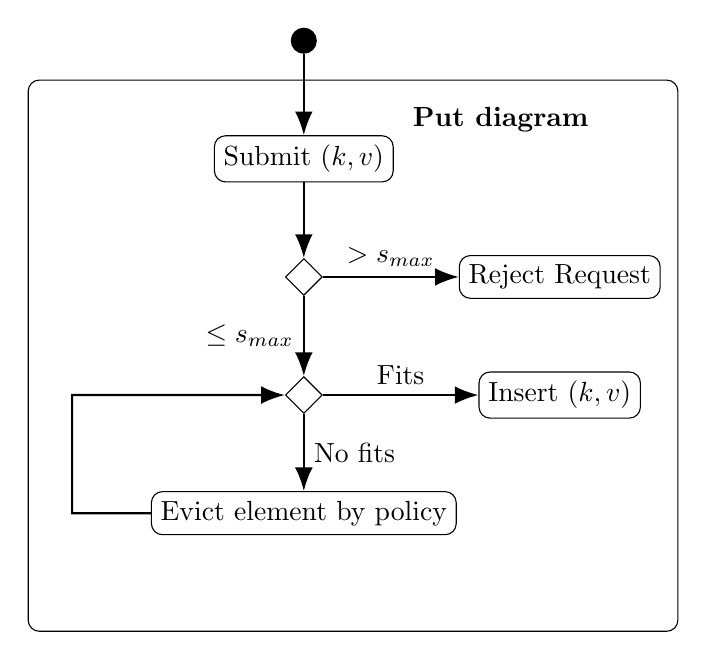
\begin{tikzpicture}[node distance=1.5cm]
        % Frame
        \draw [rounded corners] (-3.5,-1.5) rectangle (4.75, -8.5);
        \node (title) at (2.5, -2) {\textbf{Put diagram}};
        
        % Nodes
        \node[initial] (initial) at (0,-1) {};
        \node[action, below of = initial] (submit)  {Submit $(k, v)$};
        \node[decision, below of = submit] (maxCapacityDecision)  {};
        \node[action, right of = maxCapacityDecision, xshift=1.75 cm] (reject) {Reject Request};
        \node[decision, below of = maxCapacityDecision] (fitsDecision) {};
        \node[action, right of = fitsDecision, xshift=1.75 cm](insert){Insert $(k, v)$};
        \node[action, below of = fitsDecision](evict){Evict element by policy};
        \draw [arrow] (initial) -- (submit);
        \draw [arrow] (submit) -- (maxCapacityDecision);
        \draw [arrow] (maxCapacityDecision) -- (reject)node[midway, above]{$> s_{max}$};
        \draw [arrow] (maxCapacityDecision) -- (fitsDecision) node[midway, left]{$\leq s_{max}$};
        \draw [arrow] (fitsDecision) -- (insert) node[midway, above]{Fits};
        \draw [arrow] (fitsDecision) -- (evict) node[midway, right]{No fits};
        \draw [arrow] (evict.west) -- ++(-1cm, 0) -- ++(0, 1.5) -- (fitsDecision.west);
    \end{tikzpicture}
    \caption{Activity diagram for general put showing eviction.}
    \label{fig:general_put_workflow}
\end{figure}

\subsubsection{Persistency}
One main goal of this project is to have a cache that is \textit{persistent}.
We define persistency as the ability to recover the cache
after a crash or a power failure. In practice, this means the following.
Let $D$ and $DB$ be the directory and SQLite database used to initialize
the cache $X$. Assuming we store $(k, v)$ into $X$ and the program crashes,
it possible to initialize a new instance $X'$ of the same cache $X$ using the same
directory $D$ and database $DB$. Then, doing $X'.get(k)$ should return $v$.

\begin{tcolorbox}[colback=blue!5!white, colframe=blue!75!black, title=Note]
    It is theoretically possible to have two caches $X$ and $Y$ pointing
    to the same persistency $D$ and $DB$. However, this is not recommended
    because \sqlitecache~is a single-threaded cache.
\end{tcolorbox}

\subsubsection{Settings \& Recovery}
Assume that you want to reconnect to a cache $X$ that was previously
created using the same directory $D$ and database $DB$. To do so, you can
create a new instance $X'$ using the same directory and database.

Recall that our cache has three possible settings: maximum size, encryption, and compression.

The cache $X'$ will automatically detect these settings and use them. As a result,
if a developer creates $X'$ using a different set of settings, the cache will
ignore them. All settings are unique and stored
in the metadata table $(M)$. This behavior is enforced by the UNIQUE
constraint in the metadata table $(M)$ and inserting
the settings using the \texttt{ON CONFLICT DO NOTHING} clause.

%% LRUCache subsection
\subsection{LRUCache\label{sec:lru}}
The schema used for the cache table $C$ used by the LRUCache
is given by \autoref{fig:lru_cachetable_relation}. We track
recency by using the \texttt{accessed\_at} attribute. There
are not triggers that automatically update this value. Instead,
we update this value for every call to the \texttt{get(k)}
method.

During eviction, we sort the values
by the access time and evict enough items
such that a new $(k, v)$ pair can be inserted.

\begin{figure}[!htp]
    \centering
    \begin{tikzpicture}
        \umlclass[type=class]{LRUPrimaryCache}{
            key : INTEGER \\
            filename : TEXT \\
            size : INTEGER \\
            stored\_at : TIMESTAMP \\
            accessed\_at : INTEGER
        }{}
    \end{tikzpicture}
    \caption{UML class diagram for the LRUPrimaryCache relation.}
    \label{fig:lru_cachetable_relation}
\end{figure}

% LFUCache subsection
\subsection{LFUCache\label{sec:lfu}}
The schema use for the cache table $C$ is
described in \autoref{fig:lru_cachetable_relation}.
Note that we use the \texttt{accessed\_count} attribute
in $C$ to track how many times a particular key
has been accessed. However, LFUCache supports two eviction
policies: ttl based and accessed count based.

In count based eviction,
we sort the elements by their access count and
start evicting them until enough space is created
such that a new value $v$ fits into the cache.
We do not use triggers to update access counts. Instead,
we manually increment the counter whenever a key is requested.
We consider a request any moment \texttt{get(k)} gets invoked.

In ttl based eviction,
we recompute the a new ttl by
\[
ttl_{new} = ttl - (now - stored\_at)
\]
where $now$ is the current timestamp of the system.
After recomputing the new ttl, we sort the $(k, v)$
pairs until enough space becomes available to insert a new $v'$.

It is important to note that we handle expired $(k, v)$ pairs
on demand. This means that there is no background process
constantly evicting expired elements. We perform
a cleanup of expired data whenever data is requested
from the cache by using ~\texttt{get(k)}. Additionally,
we perform cleanup whenever eviction needs to take place.

\begin{figure}[!htp]
    \centering
    \begin{tikzpicture}
        \umlclass[type=class]{LFUPrimaryCache}{
            key : INTEGER \\
            filename : TEXT \\
            size : INTEGER \\
            stored\_at : TIMESTAMP \\
            accessed\_count : INTEGER \\
            ttl : REAL
        }{}
    \end{tikzpicture}
    \caption{UML class diagram for the LFUPrimaryCache relation.}
    \label{fig:lfu_cachetable_relation}
\end{figure}

%% DiskStorage subsection
\subsection{DiskStorage}
DiskStorage is a python class responsible for managing a given directory $dir$.
Under the hood, the values $v$ are stored in different files
under $dir$. Because its responsibility is to handle values,
all value oriented operations such as compression/decompression,
encryption/encryption are provided as methods on this class.

The primary motivation of having the value storage decoupled
from the primary cache in the SQLite database is the possibility
of extending value storage using a different protocol for serializing,
such as JSON.

%% Testing subsection
\subsection{Testing}
All the functionality of the \sqlitecache~package is \textbf{functionally} tested using
the \texttt{pytest} framework. The tests are located inside the \texttt{tests} directory.

We selected the pytest framework because it is the most popular testing framework
for Python. Furthermore, the isolation and lifecycle of the tests and fixtures
are well defined. This allows us to have a clean and isolated environment
for each test.


%% Simulation Subsection
\subsection{Simulation\label{sec:simulation}}
The following section describes in detail the simulation, focusing on the differences
between our methodology and the methodology used in~\cite{shah2023ImprovedCacheEviction}.

The first difference is that our cache is persistent.
The authors in~\cite{shah2023ImprovedCacheEviction} rely on the assumption
that retrieval of elements and count tracking is \textit{efficient}. Given
that they used a memory-based cache and that there was no strict definition
of efficiency, our results are expected to not be the same.

The second difference is that our cache is a key-value cache instead
of an element-oriented cache. The main difference is the hash computation.
In an element-oriented cache, the hash is computed over the element itself
while in our key-value cache, the hash is computed over the key.
As a result, instead of creating 500 unique python objects,
we draw 500 (key, value) string pairs from
\begin{equation}
D = \{(k, v) \mid k = v, k = \{\text{`001'}, \text{`002'}, \ldots, \text{`500'}\}\}
\label{eq:experiment_value_set}
\end{equation}
instead.

The third difference is the concept of \textit{size}.
The concept of cache size in~\cite{shah2023ImprovedCacheEviction}
is count based. For example, if a cache has capacity of a 100,
this means that the cache can hold up to 100 elements or
arbitrary size. As a result, let $P$ be the count capacity
of a count-sized cache. In order to find our equivalent byte-sized
cache, we can let all values be of homogenous size $b$.
Then, the byte-sized capacity $(P')$ for our cache, as defined
in~\ref{sec:size_description}, is simply
\begin{equation}
    P' = P \times b
    \label{eq:byte_capacity}
\end{equation}
Note that~\autoref{eq:experiment_value_set} defines $D$ is such a way
that~\autoref{eq:byte_capacity} holds true for our experimentation
as all values are strings of length 3.

The fourth difference is how misses are handled.
It is not clear why the
authors in~\cite{shah2023ImprovedCacheEviction}
automatically insert an element when it is missing.
A simple example of how a cache
is generally used is provided in \autoref{fig:cache_example}.

% python cache code example
\begin{figure}[ht]
    \centering
    \begin{tcolorbox}[colback=gray!5!white, colframe=gray!75!black, title=General Cache Example]
    \begin{verbatim}
if cache.get("key") is None:
    value = expensive_op()
    cache.put("key", value)
return cache.get("key")
    \end{verbatim}
    \end{tcolorbox}
    \caption{Example of cache usage in Python.}
    \label{fig:cache_example}
\end{figure}

Although \autoref{fig:cache_example}
represents a Python code snippet, the same
applies for other scenarios. For example,
a database stores pages in the buffer. When a
page fault
occurs, the database performs an I/O, which
is expensive, to retrieve the page.
Therefore, we did not include automatic
insertion of an element into the cache in
the event of a miss at the Cache classes level.

However, during simulation, we do automatic insertion
during misses. Recall that during simulation
all our (key, value) pairs have form $(k, k)$
drawn from $D$.
Therefore, if \texttt{get(k)} returns \texttt{None},
we can insert a new pair by calling \texttt{put(k, k)}.
This change makes it possible to run our simulation
as close as possible to~\cite{shah2023ImprovedCacheEviction}.

The final difference is hit and miss rates tracking.
All of our cache classes keep up-to-date hit and miss
rate statistics. This is done internally, with an I/O overhead.
Given that the HybridCache used the TTL feature
of the LFUCache, \textit{runtime} has a direct
impact. To reduce the I/O overhead
of retrieving the hit and miss rates from
the cache, we use an auxiliary in-memory hash map.
For a concise version of the simulation,
refer to Algorithm~\ref{alg:simulation}.

\begin{algorithm}
    \caption{Simulation for any given Cache}
    \label{alg:simulation}
    \begin{algorithmic}[1]
    \Require Cache $C$; Dataset $D = \{(k, v) \mid k = v, k \in \{\text{`001'}, \text{`002'}, \ldots, \text{`500'}\}\}$
    \Require $P=100$, value size $b$, and Cache capacity $P'$
    \Require $N$ total requests,
        in-memory tracking hashmap $H$
    \For{$i = 1$ to $N$}
        \State Randomly select $(k, v)$ from $D$
        \State $value \gets \text{C.get}(k)$
        \If{$value = \text{None}$}
            \State $\text{C.put}(k, v)$
        \EndIf
        \State Push hit rate, miss rate, $i$ into $H$.
    \EndFor
    \end{algorithmic}
\end{algorithm}

\section{Results and Discussion}
% Describe evaluation methodology and significant results in the evaluation section
% Evaluate the selected approach and analyze why the selected approach is good?
%   Provide an intuitive description of the algorithms, their correctness and their complexity
\subsection{Simulation Overview}
The simulation was run
on a Dell Laptop with a 11th Gen Intel(R) Core(TM) i7-11800H processor (8 cores, 16 threads)
running at 2.30GHz, 64.0 GB of installed RAM,
a 64-bit operating system with an x64-based processor, and a NVMe SSD.
We wrote the simulation
using Python3.10 and pytest as the driver.
We selected Pytest because the test-isolation generalizes
well for simulations. Therefore, simulations
are `tests' marked with the \texttt{@pytest.mark.simulation}
marker. Because running a simulation is slow,
these tests are also marked as \textit{slow}.

More importantly, we run our simulation
distributed across multiple CPUs. Given that
each simulation is isolated, we can run
all the simulations in parallel
by using pytest-xdist framework~\cite{pytestXdist}.
Additionally, pytest ships with runtime
tracking out of the box.
Refer to \autoref{fig:simulation}
for an example output of a running simulation.

\begin{figure}[!htp]
    \centering
    \includegraphics[width=\linewidth]{images/simulation_running_example.png}
    \caption{Screenshot of a running simulation.}
    \label{fig:simulation}
\end{figure}

\subsection{Simulation Details}
We let $P = 100$.
In our platform, all uncompressed and unencrypted
values in $D$ occupy $b = 18$ bytes.
Therefore, the cache size $P' = Q' = 1800$ bytes.
Furthermore, no compression and no encryption
was enabled.

The simulation was run as a sustained load
with $N = 100,000$ requests,
as described in Algorithm~\ref{alg:simulation}.
This means that the simulation runs until completion
for
$N$ requests. For example, in $N=1000$
we generate 1000 data points for both
the hit and miss rates. The duration
of each simulation run was dependent
on the eviction policy being tested.
TTL based policies, such as LFUCacheTTL
and HybridCache
took the longest. Please refer to \autoref{tab:test_simulation_metrics}
for a detailed view of the runtime of the simulations
depending on the eviction policy.

A total of four eviction policies were tested:
LRU, LFU, LFU with TTL, and Hybrid.
For any TTL based policy, we used a TTL of 5 seconds.
Finally, for the hybrid policy we set the threshold
$T = 5$. Recall that $T$ is a counter threshold
that dictates the number of times
and item is looked up before it is
moved from the LRUCache
into the LFUCache with TTL.

\subsection{Hit Rate analysis}
The results of the hit rate vs. the number
of request for each eviction policy is summarized
in \autoref{fig:hit_rate_plot}.

\begin{figure*}[!htp]
    \centering
    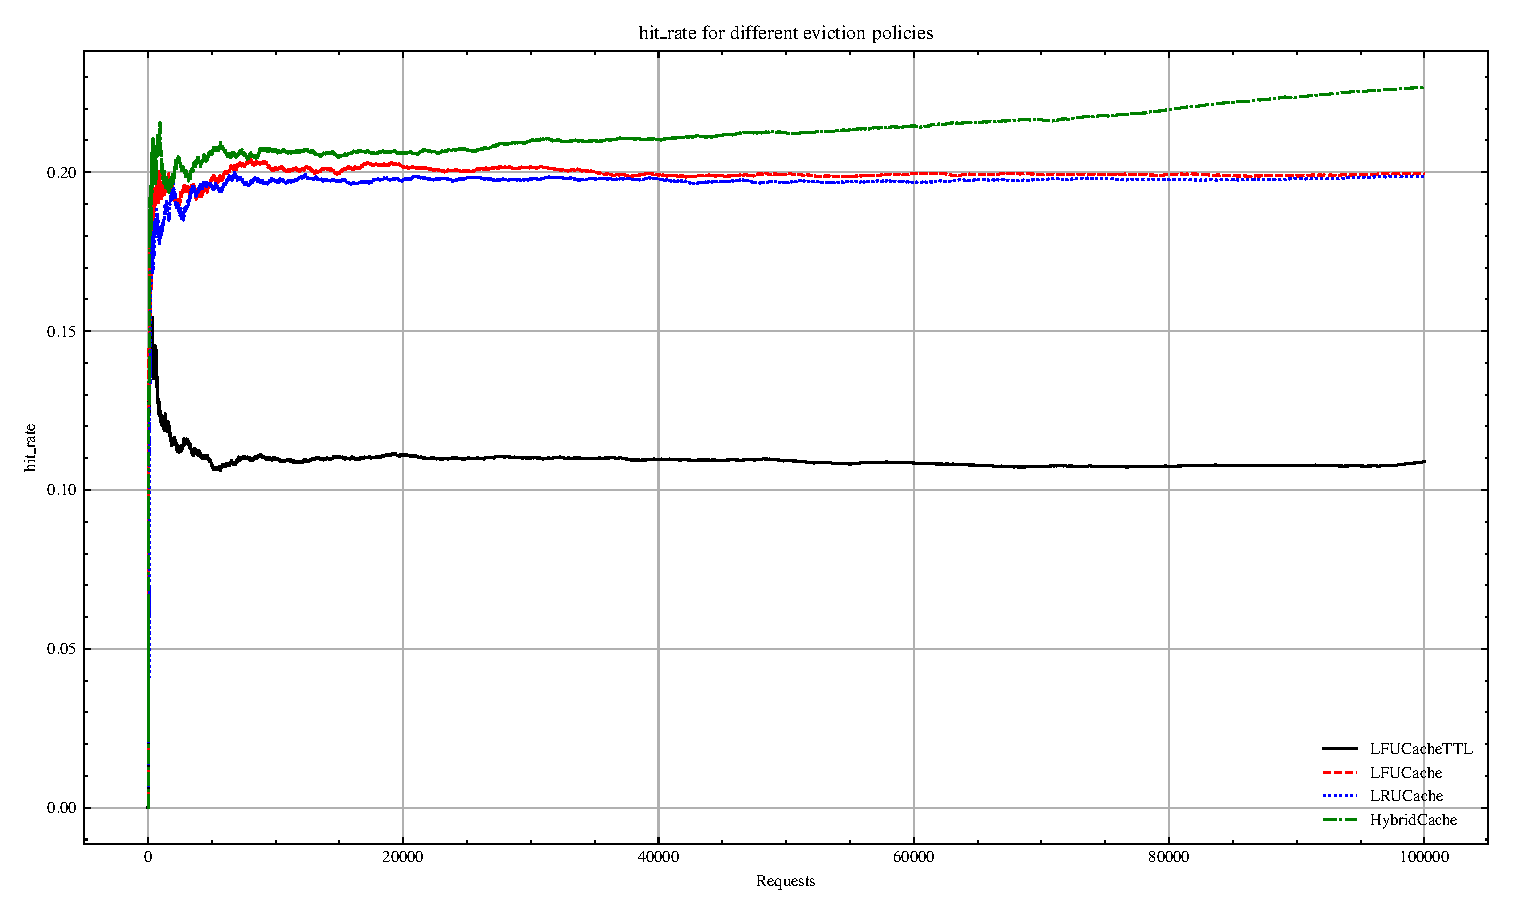
\includegraphics[width=\textwidth]{images/hit_rate_plot.eps} % Replace with the path to your EPS file
    \caption{Hit rate as a function of requests among different eviction policies}
    \label{fig:hit_rate_plot}
\end{figure*}

It is clear that the HybridCache policy performs significantly
better than all other policies across all number of requests.
The LFUCache with TTL performs the worst
among all eviction policies. These results
are in alignment with~\cite{shah2023ImprovedCacheEviction}.
Note that both the LRUCache and LFUCache eviction
policies converge at a hit rate of 20\%.
Interestingly, \[hit\_rate \approx 0.20 = \frac{100}{500} = \frac{P}{|D|}\]
which is a sign that caches converging
to $\frac{P}{|D|}$ do not generalize well as this value
is the uniform random probability of selecting $P$ items
out of a set of size $|D|$.

It is important to note that our results do not
exactly match
the ones reported in~\cite{shah2023ImprovedCacheEviction}.
We believe this is due to two reasons:

\begin{enumerate}
    \item \textbf{True randomness:} our methodology explicitly
    describes that values selected from $D$ have the same
    probability of being selected. Authors in~\cite{shah2023ImprovedCacheEviction}
    do not specify the probabilities of items drawn from $D$.
    \item \textbf{I/O Cost:} The hybrid cache
    described in~\cite{shah2023ImprovedCacheEviction}
    makes the assumption that all data structures
    and data live in memory. Given that the HybridCache
    incurs runtime penalty due to I/O, this affects
    the underlying TTL eviction. Therefore,
    it is unrealistic to expect the same results.
\end{enumerate}

Finally, note that as the number of request increases, the
difference between the hit rate of the HybridCache
and all other cache increases. This is a great sign
that the eviction policy is able to adapt to unpredictable
(random)
workloads.

\subsection{Miss Rate Analysis}

\autoref{fig:miss_rate_plot} shows the miss rate as a function
of requests for all eviction policies.
Our miss rate is defined as
\[miss\_rate = 1 - hit\_rate\]

Note that by definition, \autoref{fig:miss_rate_plot}
is the inverse of \autoref{fig:hit_rate_plot}. 
One thing to point out is that at the beginning
of the simulation, the miss rate is incredibly high.
This makes sense because at the beginning of the simulation,
the number of elements that can be possibly looked up
is significantly greater than the number of elements
currently in the cache. For example, if only
one element is currently in the cache,
the probability of that element \textbf{not being selected}
for a lookup in the cache is \[\frac{499}{500} = 0.998\].

Similar to the hit rate, the miss rate stabilizes
for most cache classes. Furthermore, the HybridCache
sees a reduction of the miss rate as the
number of requests increases \textemdash~validating
our hypothesis of adaptability.

\begin{figure*}[!htp]
    \centering
    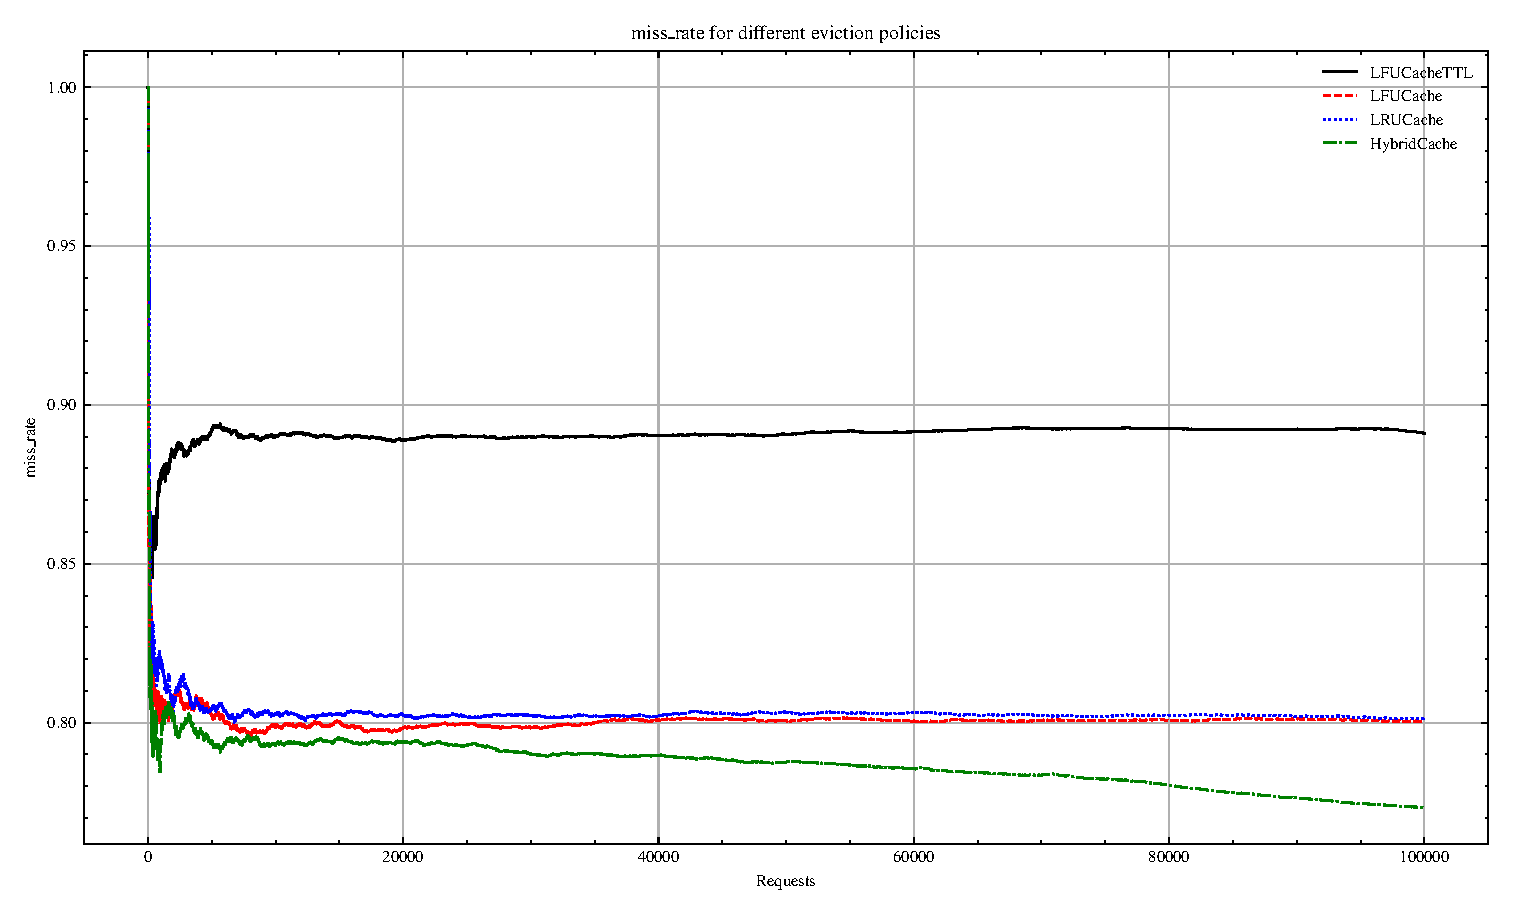
\includegraphics[width=\textwidth]{images/miss_rate_plot.eps} % Replace with the path to your EPS file
    \caption{Hit rate as a function of requests among different eviction policies}
    \label{fig:miss_rate_plot}
\end{figure*}

\subsection{Runtime Analysis}
Given the persistency of our cache implementations,
it is worth discussing the runtime differences among
them. \autoref{tab:test_simulation_metrics} summarizes
the runtime of the simulation for all the eviction policies.

\begin{table}[!htp]
    \centering
    \caption{Runtime metrics for different simulations with 100,000 requests}
    \label{tab:test_simulation_metrics}
    \begin{tabularx}{\linewidth}{XXX}
        \toprule
        \textbf{Cache} & \textbf{Runtime (s)} & \textbf{Runtime (h)} \\
        \midrule
        HybridCache & 8484.57 & 2.36 \\
        LFUCache (TTL) & 8339.01 & 2.32 \\
        LRUCache & 8190.93 & 2.28 \\
        LFUCache & 8169.70 & 2.27 \\
        \bottomrule
    \end{tabularx}
\end{table}

As expected, TTL based policies such as LFUCache with TTL,
and the HybridCache have the longest runtime. However,
when compared with the lowest runtime, these two
policies are only 2\% and 4\% slower, respectively.
Therefore, we can argue that our choice of in-demand
eviction of expired items was a smart design choice
because the runtime penalty is minimal.
\section{Conclusion\label{sec:conclusion}}
% Conclusions, lessons learned possible improvements, etc.
This project accomplished two goals. First,
we successfully implemented as single-threaded,
persistent, and high capacity key-value cache using
SQLite as a Python package: \sqlitecache.

Furthermore,
we implemented three eviction policies:
LRU, LFU, and Hybrid. Our hybrid eviction
policy was first introduced in~\cite{shah2023ImprovedCacheEviction}.
Additionally, all the functional features of our project
were functionally tested using \texttt{pytest}.
Our work with \sqlitecache~shows that it is possible to combine
relational databases and the filesystem, to effectively
take advantage of secondary storage for applications instead
of in-memory solutions. Our project is useful for workloads
where cache behavior is needed when handling
vast amounts of data.

Second, we successfully replicated the findings in~\cite{shah2023ImprovedCacheEviction}.
We used our persistent cache classes
to run a simulation to compare the hit rates and miss rates
among all eviction policies. The simulation
replicated unpredictable workloads by randomly inserting
and looking up elements drawn from a set of 500 values.
Our simulation demonstrated that the Hybrid policy
produces the highest hit rate and lowest miss rate, among all eviction policies.
These findings indicate that the policy introduced in~\cite{shah2023ImprovedCacheEviction}
can be successfully applied to persistent cache strategies
with a high degree of adaptability to unpredictable workloads.
One contribution from our project was the introduction
of a more \textit{well-defined} simulation.

By creating \sqlitecache~, we gained a deeper insight
as to how SQLite works. The \texttt{ON CONFLICT DO}~clause
was useful when dealing with settings and recovery.
Triggers were practical to accurately keep track
of the size of the cache. We believe the biggest
lesson we learned is designing a cache \textbf{that works}
by using
a set of relations. This task forced us to think
not only about how to structure data, but also how to
reuse SQL databases for building useful data structures.
Finally, by
running a simulation with I/O bound cache objects, we learned the benefits
of designing a simulation with parallelism in mind
by distributing the workload across all
available CPUs.

Although the results of our project were satisfactory,
there are several areas of improvements and expansions.

First, it will be interesting to create a multi-threaded and
distributed version of \sqlitecache.
Second, one area of expansion is to support different
serialization mechanisms besides pickle, such as JSON or
MessagePack.
Currently, our project only supports storing pickle-serializable
values inside the cache. However, pickle presents
several security risks and portability issues~\cite{arjancodesPickle}.
Third, this project can be enhanced by adding
several other eviction policies including
Most Recently Used (MRU), Random Replacement (RR),
and First In-First Out (FIFO). Fourth,
one interesting research activity will be to run
the simulation again with more eviction policies.
Finally, during our simulations, we hardcoded
the values for the counter threshold $T$ and TTL $\tau$
used by LFUCacheTTL and HybridCache. It is worth
experiment with different values for $(T, \tau)$,
either through grid search or a bayesian optimization,
and see their impact on hit rate and miss rate.
However, we acknowledge that performing parametrized
simulations or increasing the value of $N$ requests
might be challenging considering its runtime.

\bibliographystyle{IEEEtran}
\bibliography{references}

\end{document}